Den anden metode man kan bruge kaldes for et dynamisk Huffman træ. Et dynamisk træ bliver generet ud fra det reelle data som teksten består af. Træet bliver genereret ud fra den specifikke besked og er ikke en generel liste som ved den statiske metode. Det dynamiske træ er derfor den mest optimale til Huffman coding. Den dynamiske opbygning af et træ starter med at sætte de to tegn med færrest forekomster til en knude. Derefter bliver der bygget ovenpå den knude og tager hele tiden de tegn med færrest forekomster som endnu ikke er blevet sat ind i træet. En ny knude bliver lavet som får sat det næste tegn samt den foregående knude som indeholder alle tidligere tegn og knuder på.

\begin{figure}[H]
\centering
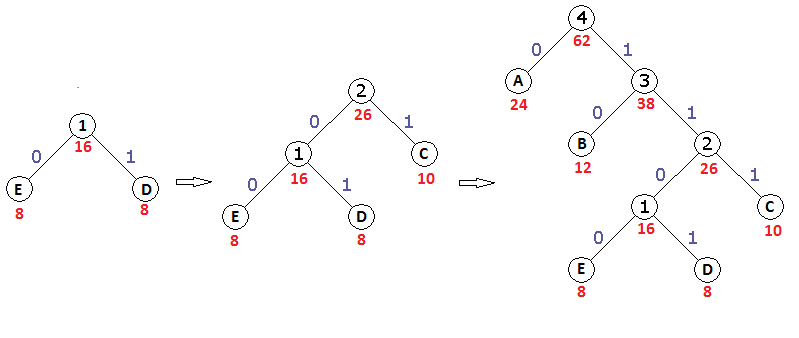
\includegraphics[width=\linewidth]{Billeder/dynamisk.png}
\caption{Dynamisk opbygning af et Huffman træ udfra det tidligere eksempel. Hentet fra binaryessence.com\cite{Hufftree_1}}
\label{fig:dynamic_tree}
\end{figure}

En ulempe ved den dynamiske metode er, at for at kunne dekode den komprimeret tekst skal man bruge en kode tabel over træet. Idet at det er et træ skræddersyet til et bestemt stykke tekst, så har dem der skal dekode teksten ingen mulighed til hvordan man oversætter 0 og 1 tallene tilbage til den oprindelige tekst. Derfor er det nødvendigt med den dynamiske metode at medsende en tabel som angiver hvilke tegn har hvilke bitmønstre. Dette betyder selvfølgelig at den komprimeret tekst fylder et stykke mere og gør derfor ikke optimalt brug af komprimeringskraften ved Huffman coding. \cite{Hufftree_4}

Fordelen ved et dynamisk træ i forhold til det statiske er at den mere konstant gør optimal brug af Huffman coding til at komprimere et stykke tekst. Det er selvfølgelig det man gerne vil opnå i forhold til SMS beskeder, men som sagt så er det nødvendigt at sende en tabel med så det er muligt at dekode det komprimeret stykke tekst. Dette betyder at SMS beskeden fylder mere end hvis det bare var det komprimeret stykke tekst, og arbejder derfor imod målet om at formindske størrelsen af den data der bliver sendt.
